\documentclass{beamer}
\usepackage[utf8]{inputenc}
\usepackage{tikz}
\usepackage{relsize}
\usetikzlibrary{shapes.geometric, arrows}
\tikzstyle{std} = [rectangle, minimum width=7cm, minimum height=0.8cm, text centered, align = center, draw=black, fill=gray!30]
\tikzstyle{arrow} = [->,>=stealth]
\newcommand{\var}{\text{var}}
\newcommand{\cov}{\text{cov}}
\newcommand{\logit}{\text{logit}}
\theoremstyle{definition}
\newtheorem{assump}{Assumption}

\addtobeamertemplate{navigation symbols}{}{%
    \usebeamerfont{footline}%
    \usebeamercolor[fg]{footline}%
    \hspace{1em}%
    \insertframenumber/\inserttotalframenumber
  }

%Information to be included in the title page:
\title{Dynamics of Consumer Demand for New Durable Goods}
\author{Gautam Gowrisanbaram, Marc Rysman \\
Presenter: Caio Figueiredo}
\institute{Penn State}
\date{2019}

\begin{document}

\frame{\titlepage}

\begin{frame}
  \frametitle{Introduction: Motivation}

  \begin{itemize}
    \item In many durable goods setting, the choice of when to buy is as important
      as what to buy
    \item This is specially true for consumer electronics, since prices are
      expected to fall during the its lifetime
  \end{itemize}
\end{frame}

\begin{frame}
  \frametitle{Introduction: Objective}

  Objective:
  \begin{itemize}
    \item Specify a structural dynamic model of consumer
      preferences for new durable goods,
    \item Estimate the model using data on digital recorders,
    \item Use model to evaluate elasticities and cost-of-living indices for
      this market.
  \end{itemize}
\end{frame}

\begin{frame}
  \frametitle{Introduction: The Market}

  \begin{itemize}
  \item About 11 million units of camcorders were sold in the U.S. from 2000 to
    2006,
  \item During this time the average price dropped from \$930 to \$380,
  \item Meanwhile, the average pixel count rose from 580k to 1.08m,
  \item The number of models grew from less than 30 to almost 100,
  \item and the average sales grew by a factor of 2.6.
\end{itemize}
\end{frame}

%\begin{frame}
  %\frametitle{Introduction: The model}

  %\begin{itemize}
    %\item Camcorders are durable and provide a flow of utility into the future,
    %\item The available prices, quality and variety may improve over time, so
      %waiting can be valuable,
    %\item To make the problem tractable this is assumed to follow a Markov
      %process.
    %\item Consumers can only held one camcorder at a time,
    %\item Consumer continues to evaluate the market even after the purchase,
  %\end{itemize}
%\end{frame}

%\begin{frame}
  %\frametitle{Introduction: COLIs}

  %\begin{itemize}
    %\item The use of COLI (Cost of Living Index) are necessary in order to
      %accurately measure welfare level.
    %\item CPI (consumer price index) computed by the Bureau of Labor Statistics
      %is often used as COLI, but this have undesired implications.
    %\item CPI would show welfare substantially improving since prices fall and
      %quantities rise.
    %\item However, if high-value consumers purchase early and low-value
      %consumers purchase late, standard approaches will overstate the welfare
      %gains.
    %\item This problem is avoided by the dynamic nature of this model, where
      %later buyers will either be low values types or already hold the good.
  %\end{itemize}
%\end{frame}

\begin{frame}
  \frametitle{Model}
  
  \begin{itemize}
    \item The industry starts at time $t = 0$,
    \item The consumer has infinite horizon and discounts the future at rate
      $\beta$
    \item The consumer can benefit from at most one camcorder in a period,
    \item There is no resale market, if the consumer choose to change his
      camcorder, the old one is discarded costlessly.
  \end{itemize} 

\end{frame}

\begin{frame}
  \frametitle{Model}

  The utility of each camcorder $j$ at time $t$ is:

  \[ u_{jt} = f_{jt} - P_{jt} + \varepsilon_{jt}\text{, for }j = 1,\ldots J_t \]

  Where:

  \begin{itemize}
    \item $f_{jt}$ is the net flow utility of camcorder $j$ at time $t$,
    \item $P_{jt}$ is the disutility of price of camcorder $j$ at time $t$,
    \item $\varepsilon_{jt}$ is the idiosyncratic type 1 extreme value term,
      distributed \textit{i.i.d.} across models and time periods.
  \end{itemize}

\end{frame}

\begin{frame}
  \frametitle{Model}

  \begin{itemize}
    \item A consumer who does not purchase any model at time $t$ receives $u_{0t} =
      f_{0t} + \varepsilon_{0t}$,
    \item Where $f_{0t}$ is the flow utility of the good that the consumer
      possess at time $t$,
    \item If the consumer possess the outside good then $f_{0t} = 0$.
    \item Finally the consumer chooses $j$ that has the maximum utility.
  \end{itemize}
\end{frame}

\begin{frame}
  \frametitle{Model}

  Therefore, the consumer value function can be written as:

  \begin{align}
    V(f_0, \Omega) = \int \max \bigg\{& f_0 + \beta
    \mathop{\mathbb{E}} [V(f_0,\Omega')|\Omega] + \varepsilon_0, \\
    & \max_{j = 1,\ldots ,J} \{f_j -P_j + \beta
    \mathop{\mathbb{E}} [V(f_j, \Omega')|\Omega] + \varepsilon_j\}\bigg\}
    g_{\vec{\varepsilon}}(\vec{\varepsilon})d\vec{\varepsilon}
  \end{align}

  Where:
  \begin{itemize}
    \item $\vec{\varepsilon} \equiv (\varepsilon_0, \ldots,
    \varepsilon_{J_tt})$
    \item Primes (e.g. $\Omega'$) denotes the next period value of a variable.
    \item The state evolves according to some Markov process: $g_{\Omega} =
      (\Omega_{t+1}|\Omega_t)$.
  \end{itemize} 
\end{frame}

\begin{frame}
  \frametitle{Model}

  \begin{itemize}
    \item $\Omega_t$ denote the current industry state and includes: The number
      of models $J_t$, the price disutility and mean flow utility for each
      model, and any other factor that influence future model attributes,
    \item $\Omega$ has a very large dimension resulting in a curse of
      dimensionality,
  \end{itemize}

\end{frame}

\begin{frame}
  \begin{itemize}
    \item In order to get around this we proceed by using the aggregation
      properties of the extreme value distribution to express the previous
      equation as:
  \end{itemize}

  \[
    V(f_0, \Omega) = \ln [ \exp (f_0 + \beta
    \mathop{\mathbb{E}}[V(f_0, \Omega')|\Omega]) +
    \exp(\delta(\Omega))]
  \]

  Where $\delta(\Omega)$ is defined as:

  \[
    \delta(\Omega) = \ln \left( \sum_{j = 1, \ldots, J} \exp (f_j - P_j + \beta +
      \mathop{\mathbb{E}}[V(f_0, \Omega')|\Omega])\right)
  \]
\end{frame}

\begin{frame}
  \frametitle{Model}
  
  We further simplify the process by assuming:

  \begin{assump}
    \textit{Inclusive Value Sufficiency (IVS)}: \\ If $\delta(\Omega) =
    \delta(\tilde \Omega)$, then $g_{\delta}(\delta(\Omega')|\Omega) =
    g_{\delta}(\delta(\tilde \Omega')| \tilde \Omega)$ for all $\Omega, \tilde
    \Omega$.
  \end{assump}

  \begin{itemize}
    \item The IVS assumption imply that all states with the same
      $\delta(\Omega)$ have the same expected value,
    \item Thus, it is sufficient for the consumer to track only two scalar
      variables: $f_0$ and $\delta$.
  \end{itemize}

\end{frame}

\begin{frame}
  \frametitle{Model}

  Finally, we rewrite the problem as:

  \[
    \mathcal{V}(f_0, \delta) = \ln [ \exp (f_0 + \beta
    \mathop{\mathbb{E}}[\mathcal{V}(f_j, \delta')|\delta]) +
    \exp(\delta)]
  \]

  \[
    \delta = \ln \left( \sum_{j = 1, \ldots, J} \exp (f_j - P_j + \beta +
      \mathop{\mathbb{E}}[\mathcal{V}(f_j, \delta')|\delta])\right)
  \]

\end{frame}

\begin{frame}

  We also assume that the consumer has a limited ability to predict future
  model attributes, we say:

  \[
    \delta_{t+1} = \gamma_1 + \gamma_2 \delta_t + \nu_{t+1}
  \]
  
  Where
  
  \begin{itemize}
    \item $\gamma_1$ and $\gamma_2$ are incidental parameters,
    \item $\nu_{t+1}$ is normally distributed with mean $0$ and unobserved at 
      time $t$.
    \item Note that this implies that if $ 0 < \gamma_2 < 1 $
  \end{itemize}

\end{frame}

%\begin{frame}
  %\frametitle{Model}

  %\begin{itemize}
    %\item But how truthful are these assumptions?
    %\item The authors run a Monte Carlo simulation, to conclude: Very.
  %\end{itemize}

  %\begin{figure}
    %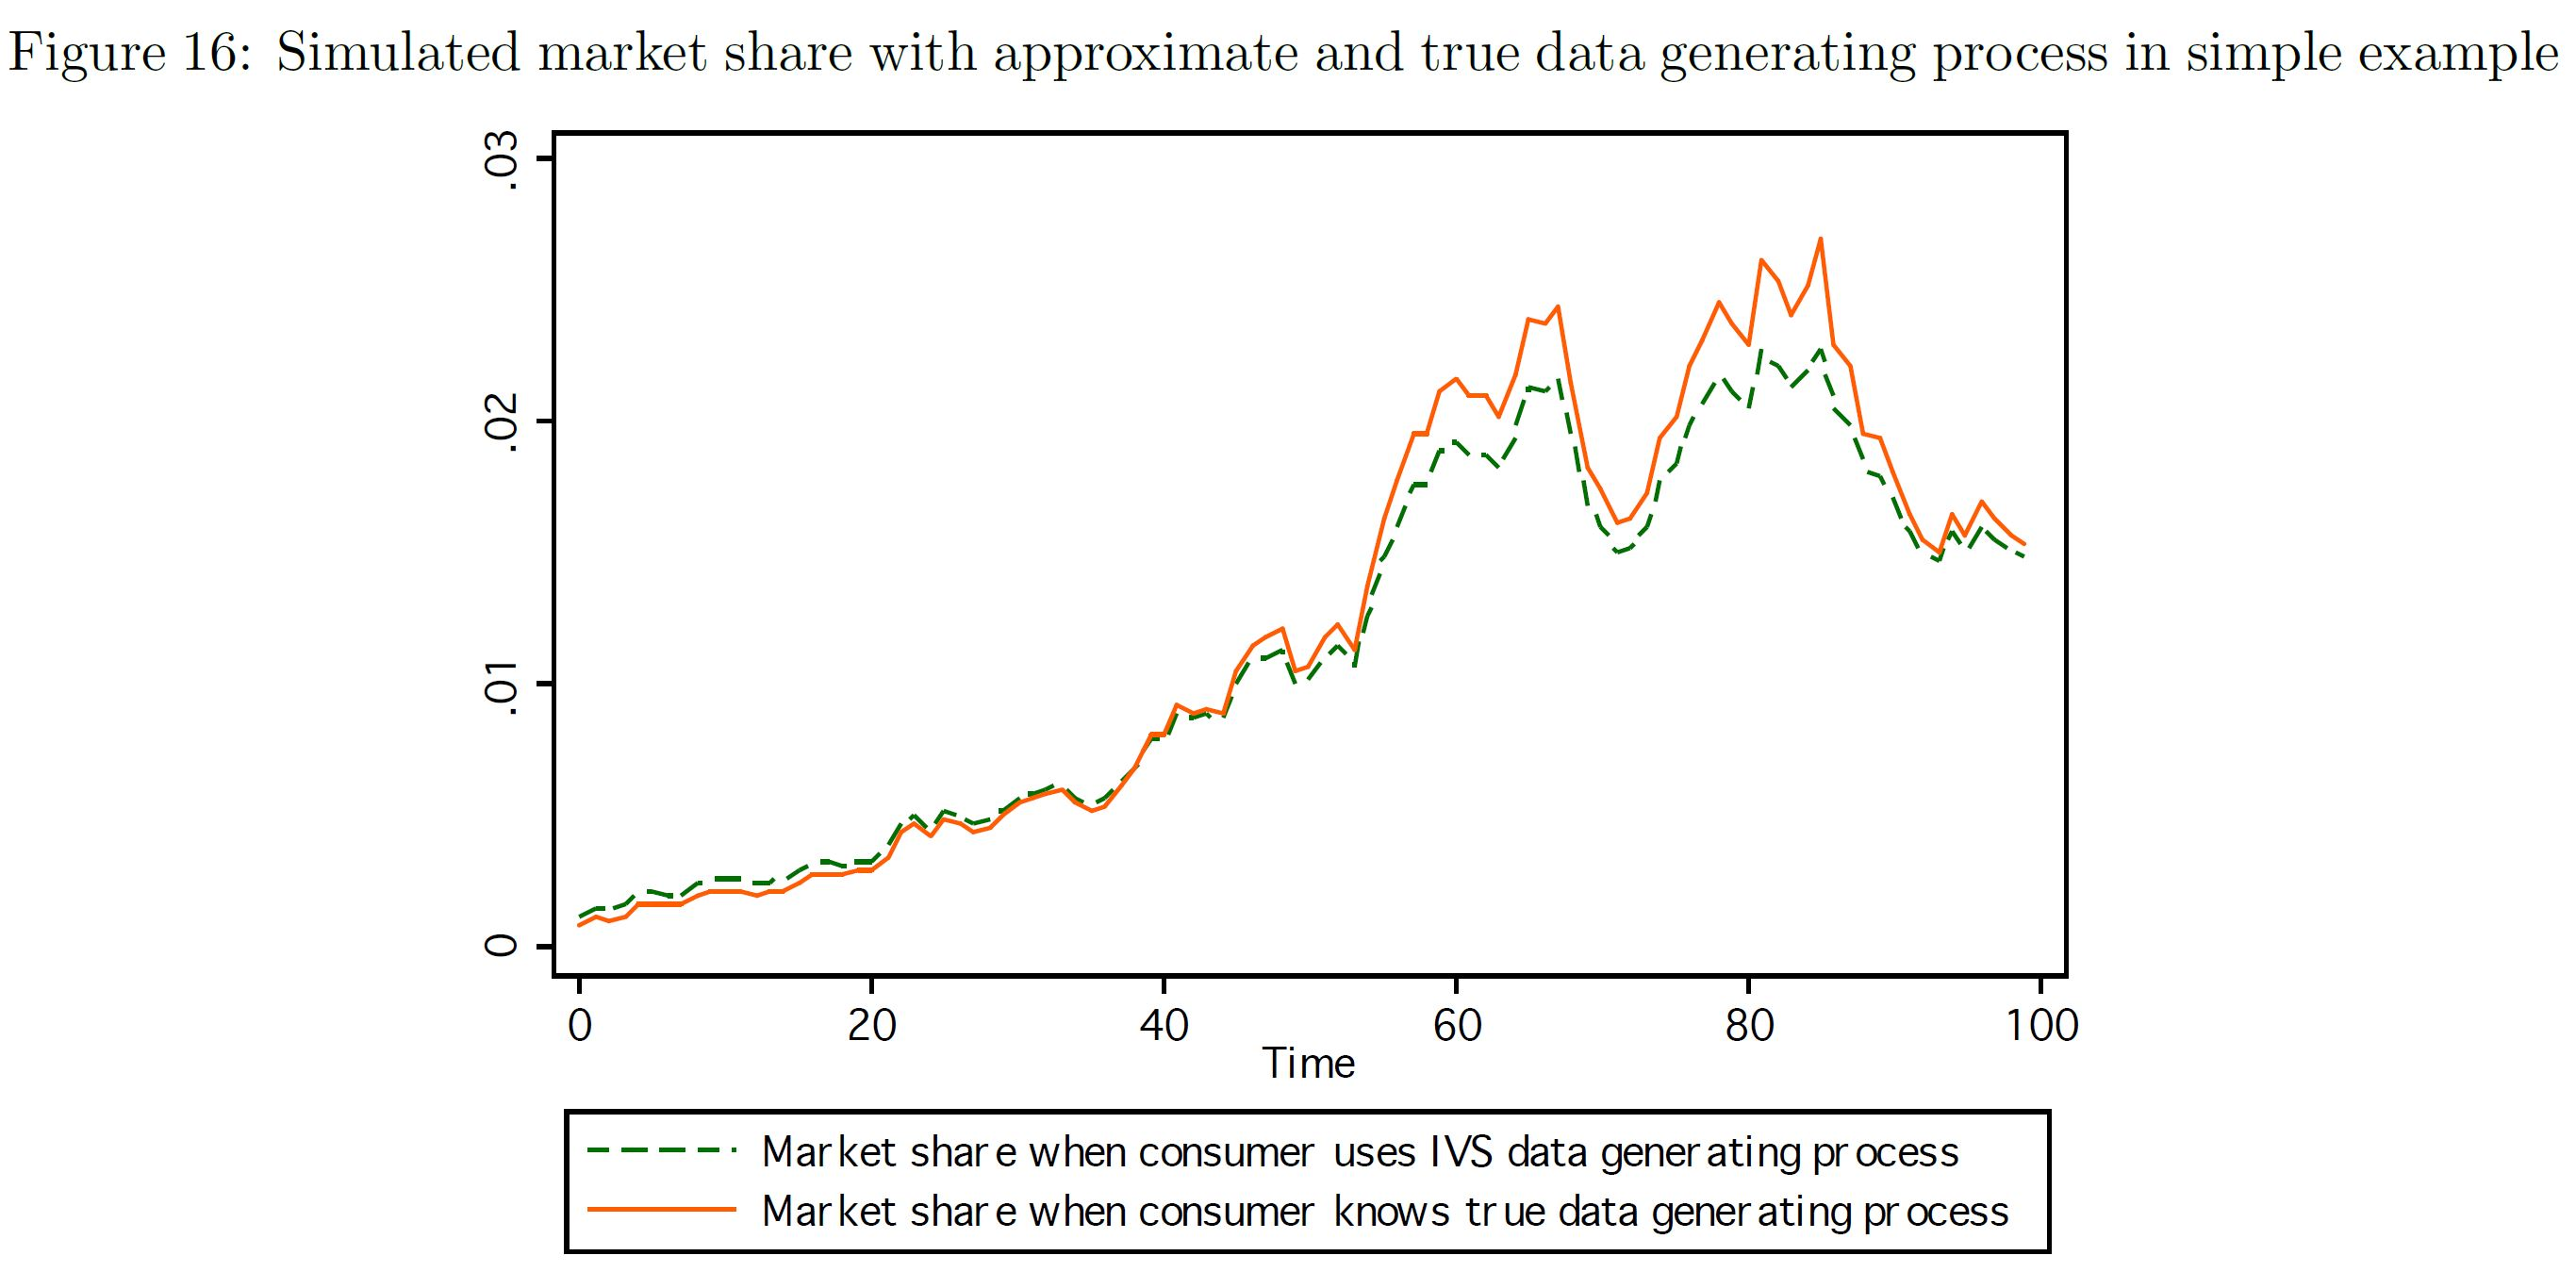
\includegraphics[width=\linewidth]{16.JPG}
  %\end{figure}
%\end{frame}

\begin{frame}
  \frametitle{Aggregation}

  \begin{itemize}
    \item Until now we have considered the decision of a single consumer to continue
      we have to define individuals characteristics and aggregate,
    \item Consumers differ in their mean flow utility, disutility of price,
      idiosyncratic shocks, logit inclusive values, Bellman Equation, and
      expectations processes for the future.
    \item That is, those terms are indexed by $i$: $f_{ijt}, P_{ijt},
      \varepsilon_{ijt}, \delta_{ijt}, \mathcal{V}_{ijt}, \gamma_{1i},
      \gamma_{2i}, \nu_{it}$.
  \end{itemize}
\end{frame}

\begin{frame}
  \frametitle{Aggregation}

  Individual net flow utility for model $j$ at time $t$ is:

  \[f_{it} = x_{jt} \alpha_i^x + \xi_{jt}\]

  Where:
  \begin{itemize}
    \item $ x_{jt}$ is observed characteristics of camcorder,
    \item $\xi_{jt}$ is unobserved characteristics, our error term,
    \item $\alpha_i^x$ are consumer $i$'s coefficients on observed characteristics.
  \end{itemize}
\end{frame}

\begin{frame}

  Price disutility is given by:
  
  \[ P_{ijt} = \alpha^p_i \ln(p_{jt}) \]

  Where $\alpha^p_i$ is the price coefficient and $p_{jt}$ is price.

  \begin{itemize}
    \item We define $\alpha_i = (\alpha^x_i, \alpha^p_i)$ to simplify notation,
    \item and say that \textbf{$\alpha_i$ has mean $\alpha$ and variance
        $\Sigma$}.
  \end{itemize}
\end{frame}

\begin{frame}
  \frametitle{Supply}

  \begin{itemize}
    \item For the supply side, we assume that models arrive according to some
      exogenous process and that their characteristics evolve exogenously as well,
    \item After observing consumer endowments, $x_{jt}$ and $\xi_{jt}$ for all
      current models, firms simultaneously make pricing decisions in a Markov
      Perfect Equilibrium,
    \item Firms cannot commit to prices beyond the current period.
  \end{itemize}
\end{frame}

\begin{frame}
  \frametitle{Inference}

  In order to make inference, we define the aggregation as follows:

  \[
    F_{jt} = x_{jt}\alpha^x + \xi_{jt}, j = 1, \ldots, J_t
  \]

  \begin{itemize}
    \item Note that: $f_{ijt} = F_{jt} + (\alpha_i^x - \alpha^x)x_{jt}$
    \item and $(\alpha_i^x - \alpha^x) \sim N(0, \Sigma)$
  \end{itemize}

\end{frame}

\begin{frame}
  \frametitle{Beta is 0.99}

  {\huge Beta = 0.99}

\end{frame}

\begin{frame}
  \frametitle{Inference}

  \begin{itemize}
    \item Following BLP we have the following GMM criterion function:
  \end{itemize}

  \[
    G(\alpha, \Sigma) = z' \vec{\xi}(\alpha, \Sigma)
  \]

  And therefore our estimatives are defined by:

  \[
    \left( \hat{\alpha}, \hat{\Sigma} \right) = \arg\min_{\alpha, \Sigma}
    \left\{ G(\alpha, \Sigma)'WG(\alpha, \Sigma)\right\}
  \]
\end{frame}

\begin{frame}
  \frametitle{Inference}

  In order to calculate $\vec{\xi}(\alpha, \Sigma)$, we need to solve the
  market shares, which are given by the consumer maximization problem.

  The \textit{conditional probability of purchase} is defined as:

  \[
    \frac{\exp (\delta_{it})}{\exp (\mathcal{V}_i(f_{i0t}, \delta_{it}))}
    \times
    \frac{ \exp (f_{ijt} - P_{ijt} + \beta
      \mathop{\mathbb{E}} [\mathcal{V}_i(f_{ijt}, \delta_{i, t+1})|
        f_{ijt}, \delta_{it}])}
      { \exp(\delta_{it}) }
  \]
\end{frame}

\begin{frame}
  \frametitle{Inference}

  \begin{itemize}
    \item We now match the predicted market share with the data, by doing to following
      interactive process:
    \item Start at $t = 0$ with $s_{00} = 1$. Everyone holds the outside good,
    \item Update conditional probability of purchase according to previous
      equation until fixed point,
    \item integrate of consumers to find market share.
    \item Choose $\vec{F}$ in order to match predicted values with data. That is:

      \[
        s_{jt} = \hat{s}_{{jt}}\left(\vec{F}, \alpha^p, \Sigma\right),\ \forall\ j,t
      \]
  \end{itemize} 
\end{frame}

\begin{frame}{Inference}

  We update $\vec{F}$, by the following process:

  \[
    F_{jt}^{\text{new}} = F_{jt}^{\text{old}} + \psi \cdot \left(
      \ln(\hat{s_{jt}}) - \ln \left( \hat{s}_{jt}\left( \vec{F}^{\text{old}},
          \alpha^p, \Sigma \right) \right) \right),\ \forall\ j,t
  \]

  Where $\psi$ is a tunning parameters set to $1 - \beta = 0.01$.
\end{frame}

\begin{frame}
  \frametitle{Inference}

  \begin{itemize}
    \item Authors can't prove that these equations have a unique fix point,
    \item But different starting values were used and have always obtained
      convergence to the same solution.
    \item Therefore the following is being assumed:
  \end{itemize}

  \begin{assump}
    For any vector of parameters ($\alpha^p, \Sigma$), there is a unique vector
    $\vec{F}$ such that $\vec{s} = \vec{\hat{s}}\left(\vec{F}, \alpha^p,
      \Sigma\right)$.
  \end{assump}
\end{frame}

\begin{frame}[t]{Identification}
  \begin{itemize}
    \item The increase in market share of model $ j$ associated with a change
      in a characteristic of $ j$ identifies the mean of $\alpha$,
    \item The models from which $ j$ draws markets shares identify $\Sigma$,
    \item In order to identity the extent of repeat purchasing, additional 
      household survey data is used.
\end{itemize}
\end{frame}

\begin{frame}
  \frametitle{Data}

  \begin{itemize}
    \item The primary data source in a panel of model-level data for digital
      camcorders, collect by NPD Techworld, which covers 80\% of the market
    \item We observe 383 models and 11 brands, monthly, from March 2000 to May 2006,
    \item For each model at each month we observe price, number of units sold and
      other characteristics.
    \item Outliers, such as product with very low sales, very high or very low prices
      are excluded. Less then 3\% of the date is excluded this way.
  \end{itemize}
\end{frame}

\begin{frame}
  \frametitle{Data - Number of models increases}

  \begin{figure}
    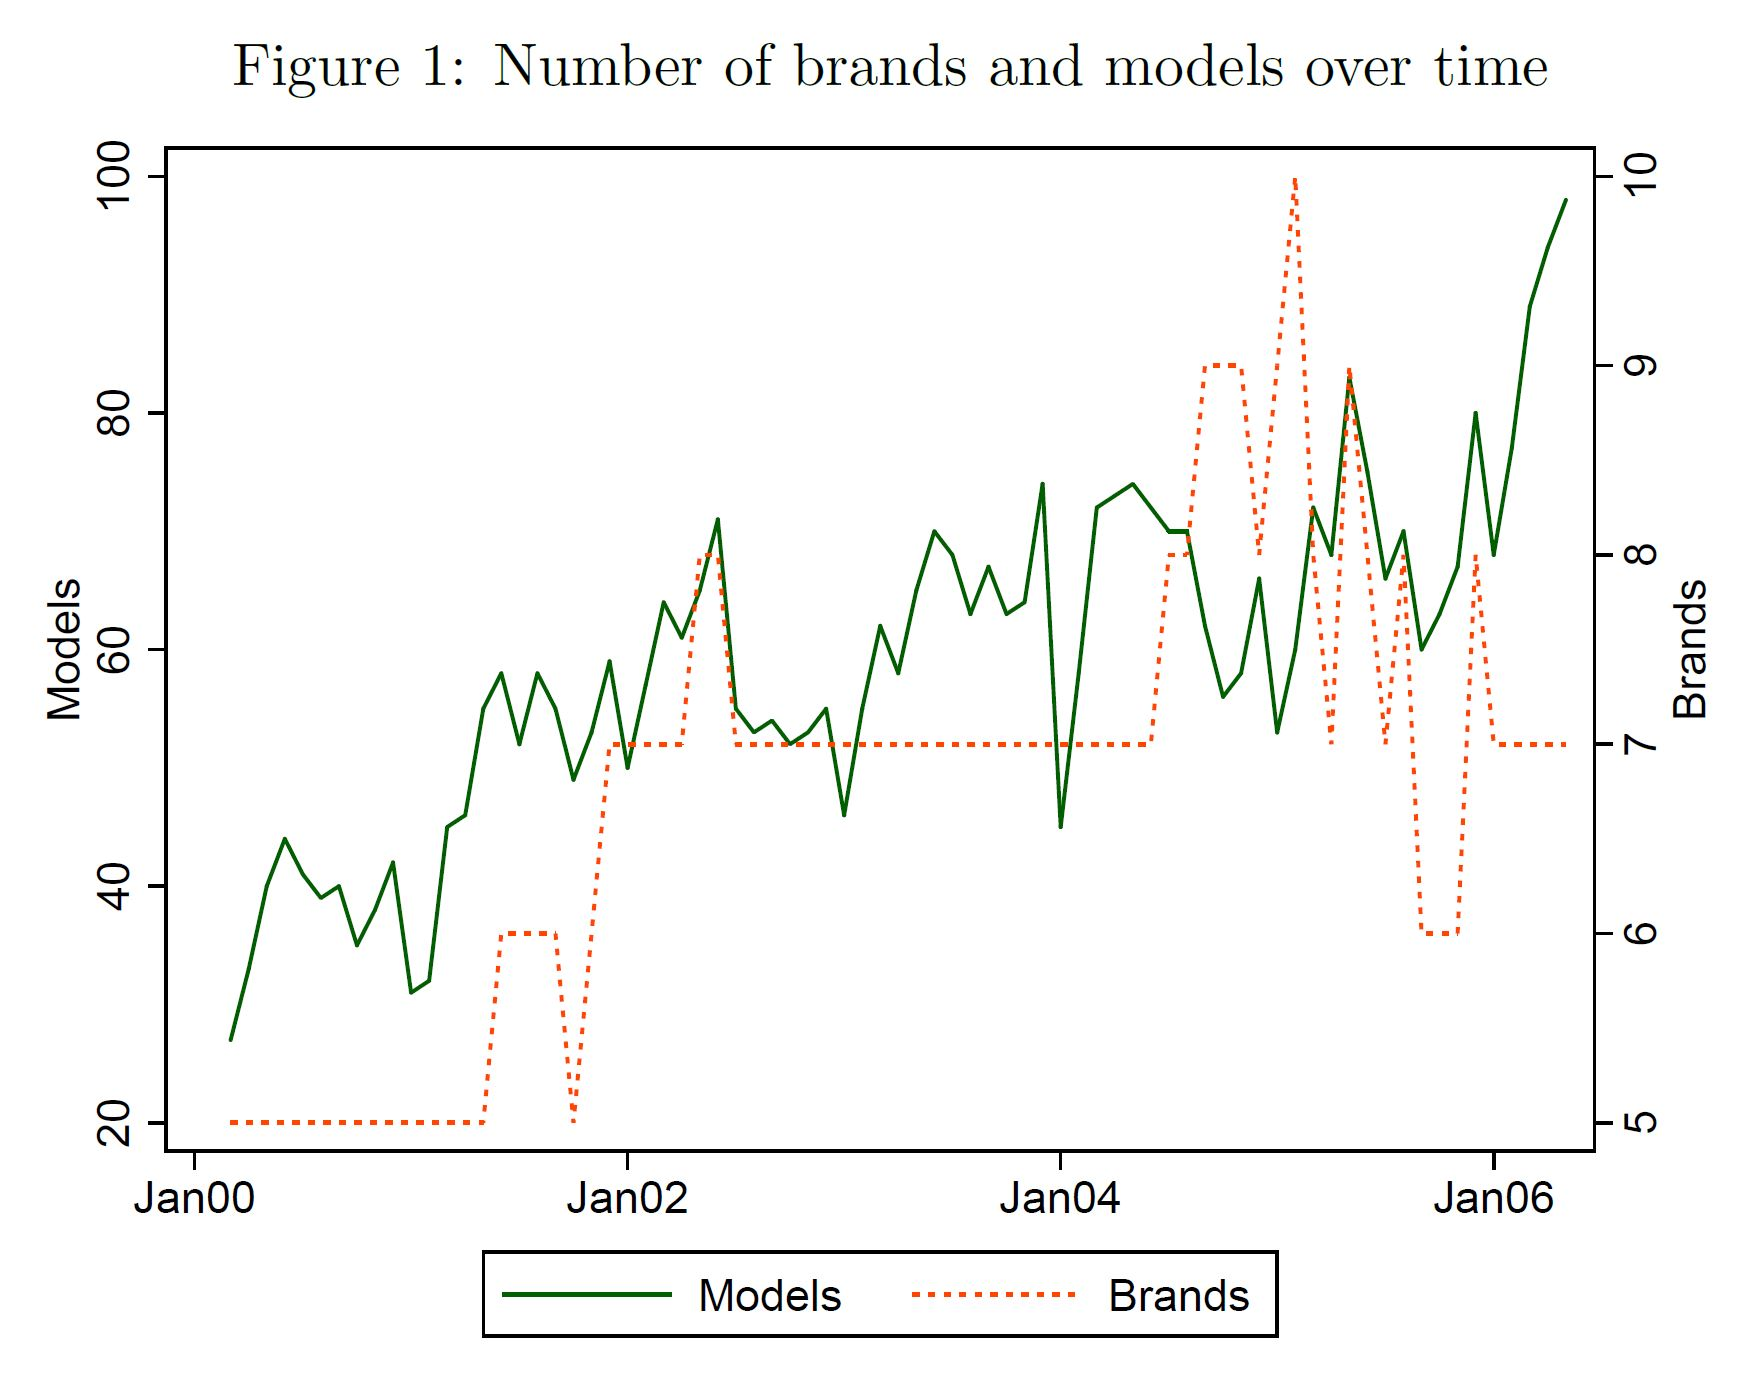
\includegraphics[width=\linewidth]{1.JPG}
  \end{figure}
\end{frame}

\begin{frame}
  \frametitle{Data - Prices falls sales increases}

  \begin{figure}
    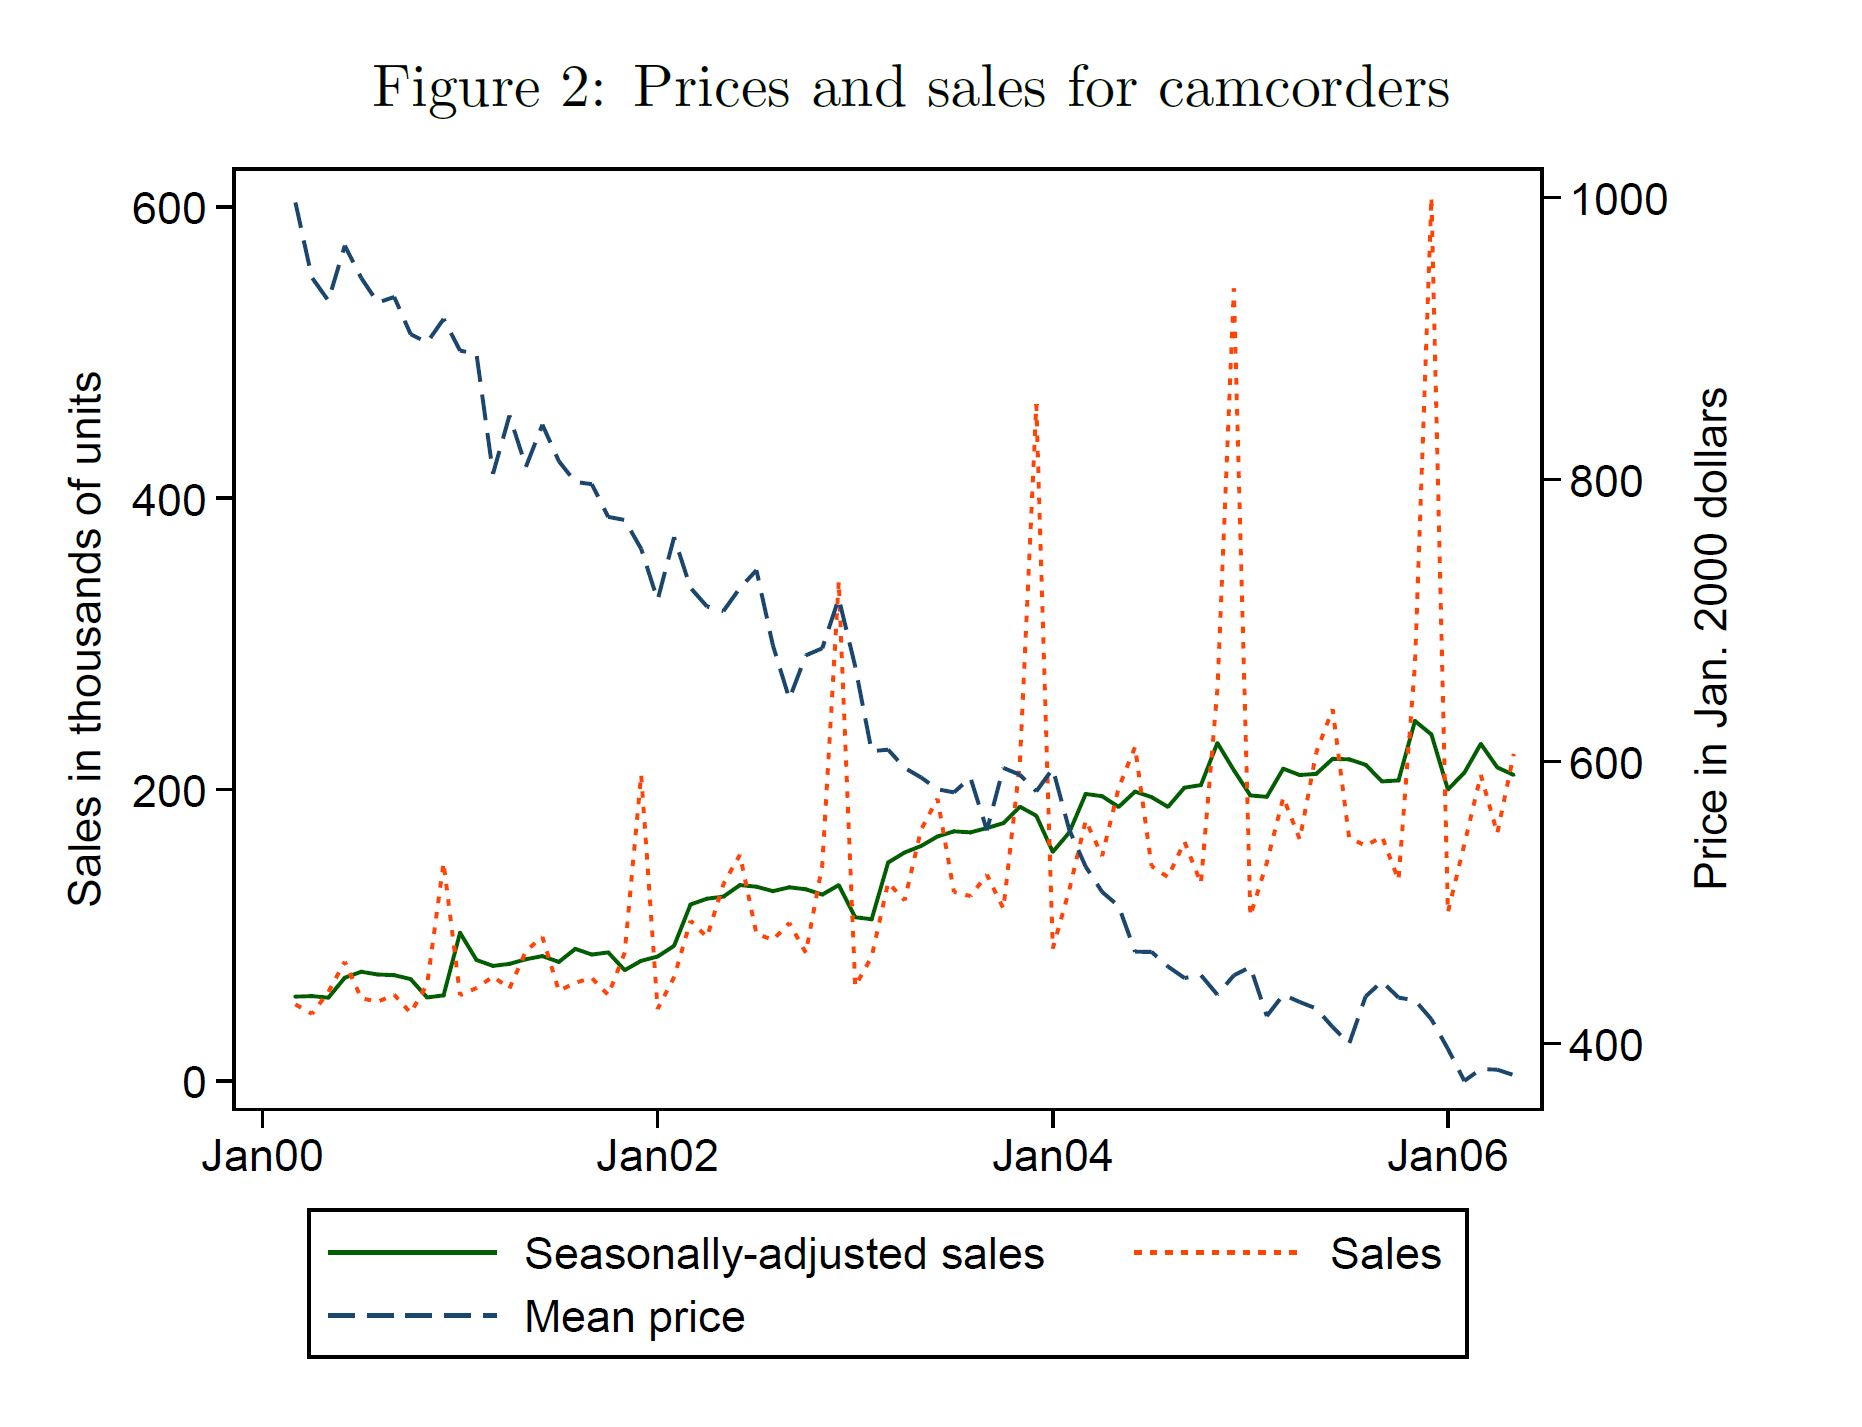
\includegraphics[width=\linewidth]{2.JPG}
  \end{figure}
\end{frame}

\begin{frame}
  \frametitle{Data - Characteristics improve over time}

  \begin{figure}
    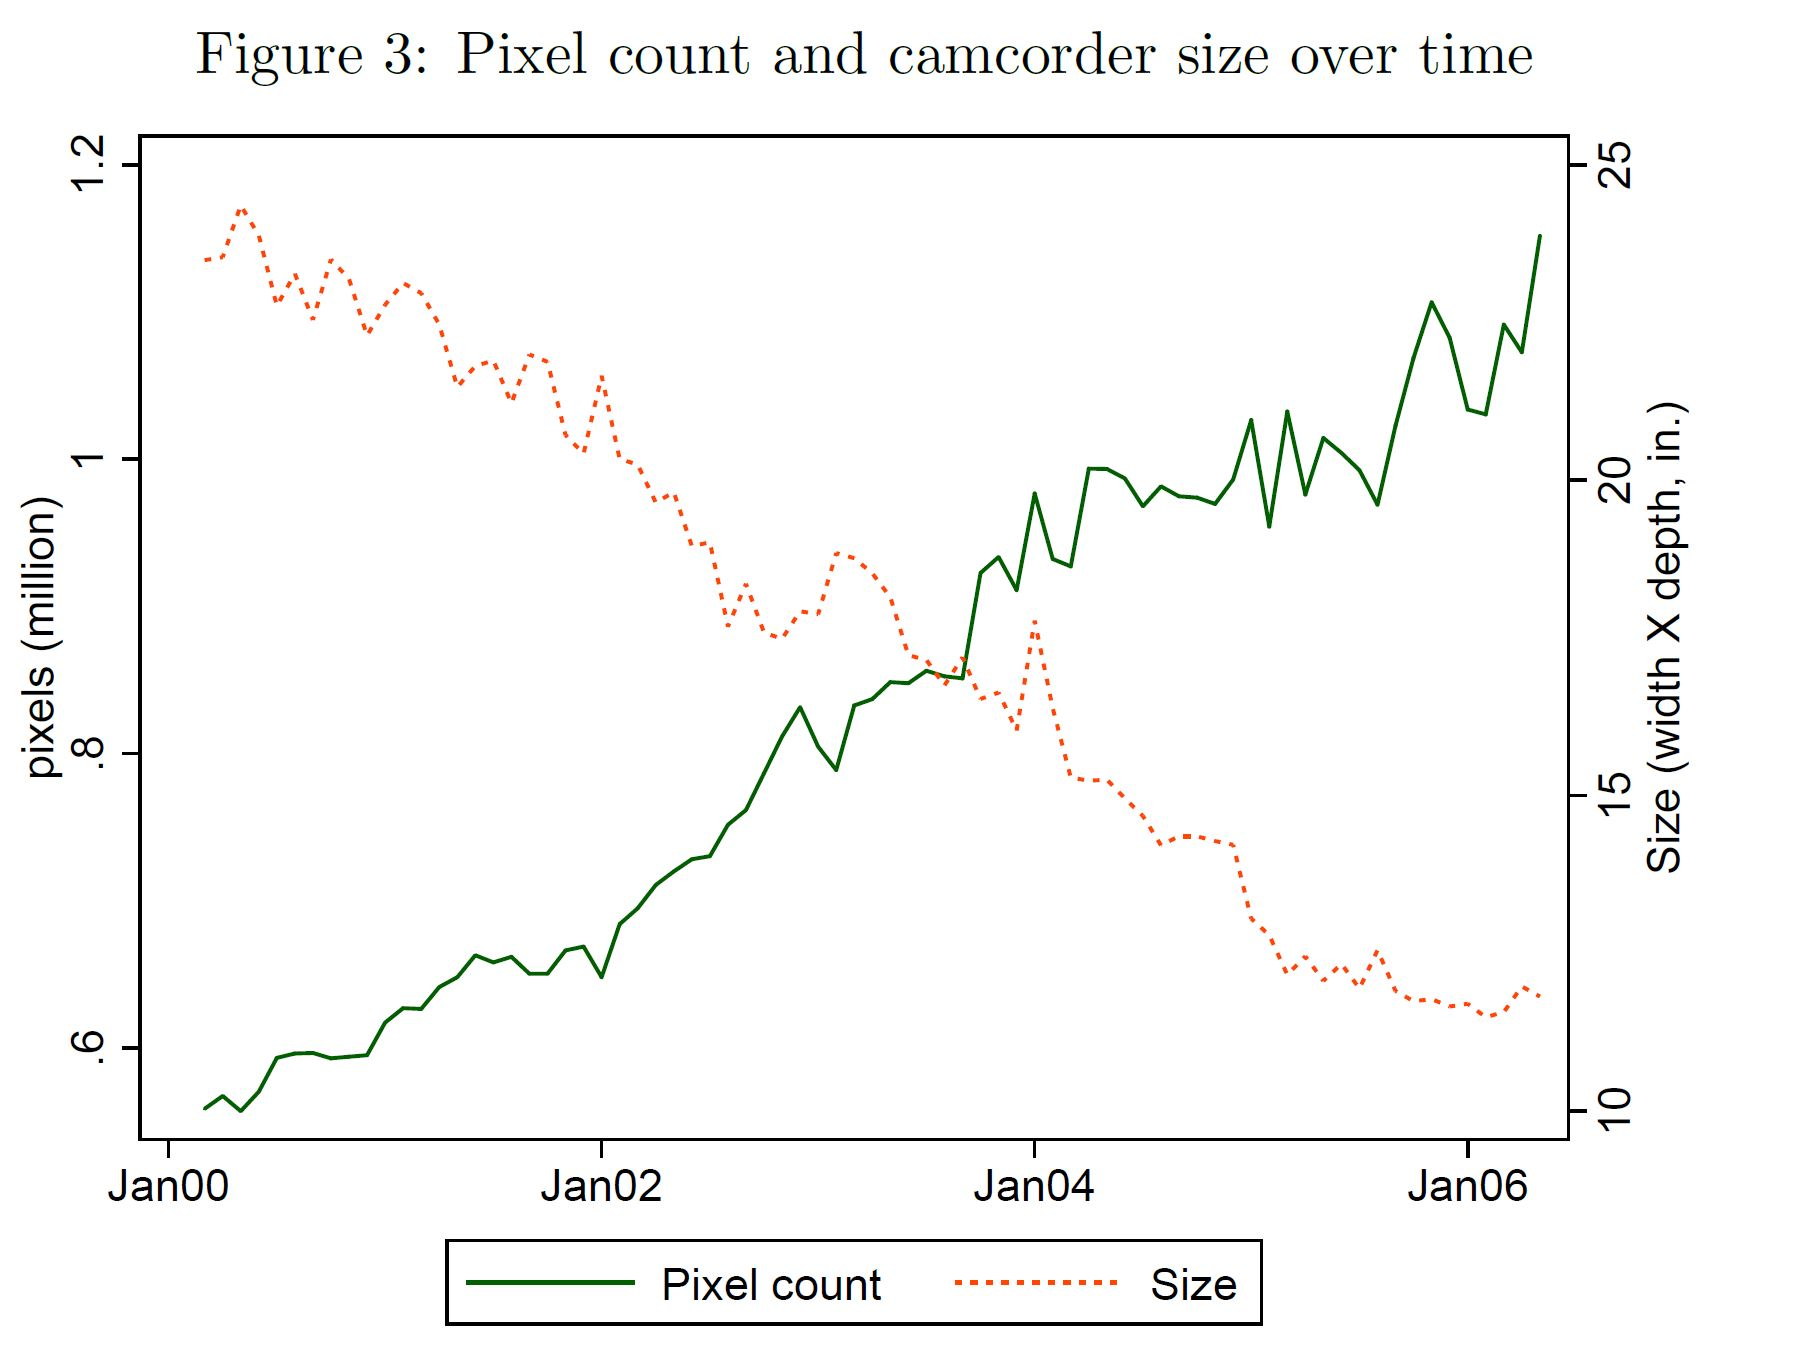
\includegraphics[width=\linewidth]{3.JPG}
  \end{figure}
\end{frame}

\begin{frame}
  \frametitle{Data - Media Type}

  \begin{figure}
    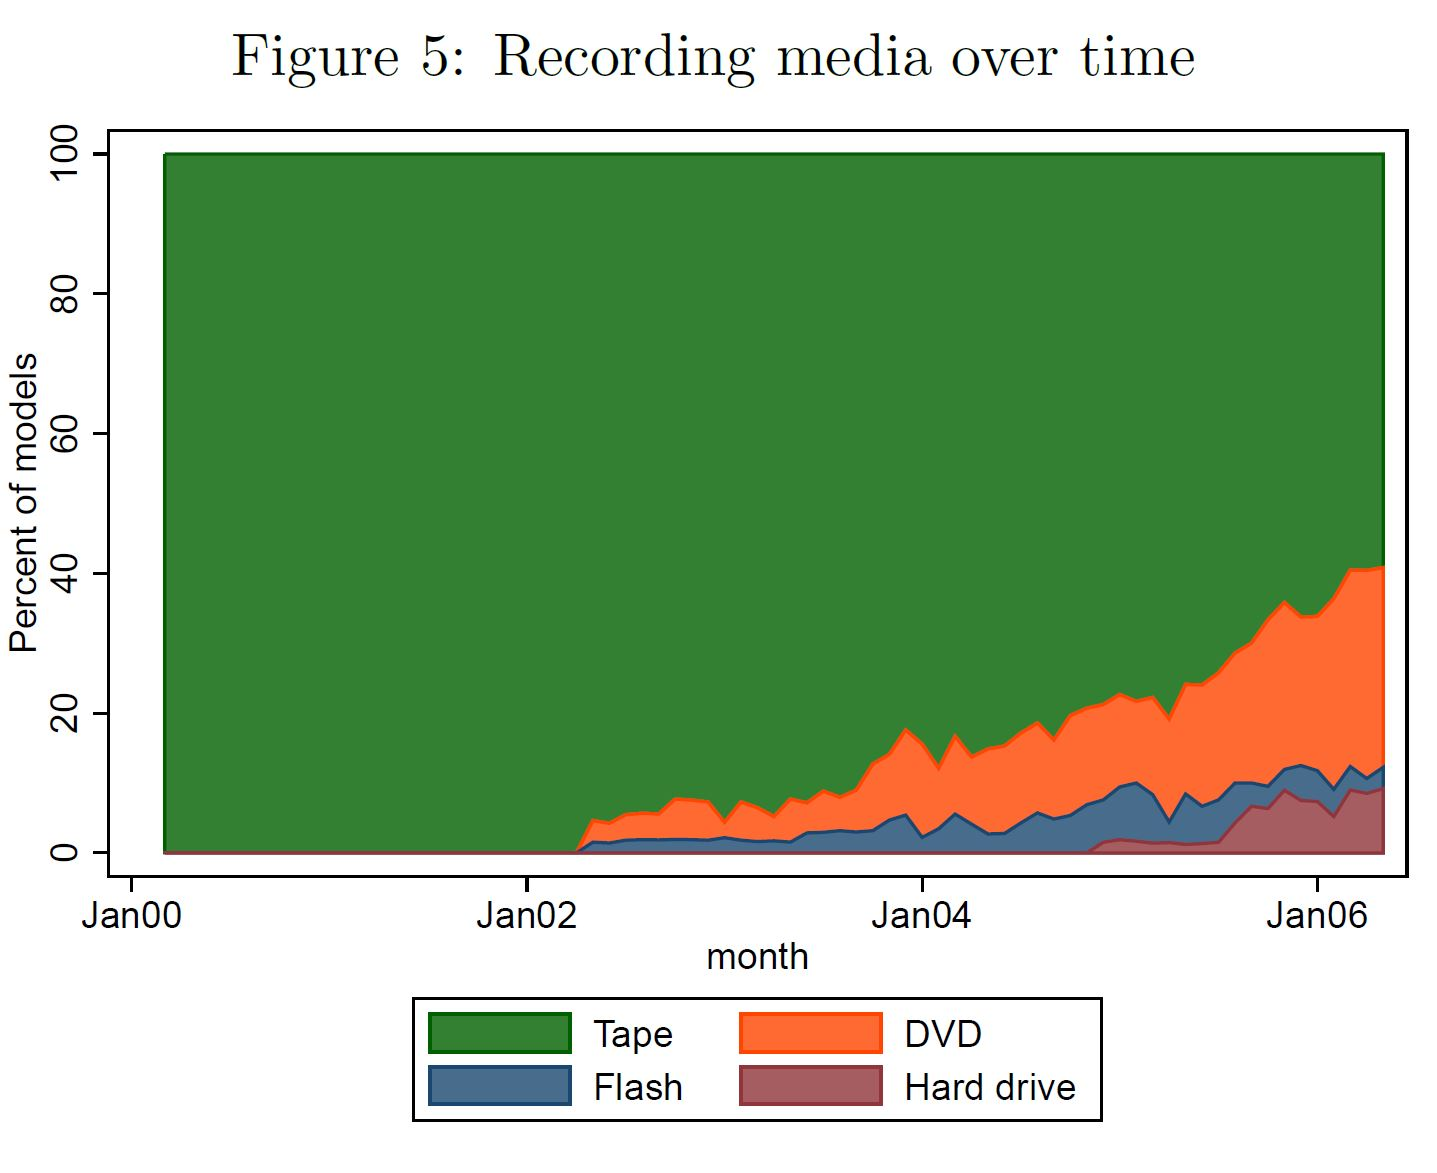
\includegraphics[width=\linewidth]{5.JPG}
  \end{figure}
\end{frame}

\begin{frame}
  \frametitle{Data - ICR-CENTRIS}

  \begin{itemize}
    \item Finally ICR-CENTRIS data is used to identify repeated purchase. 
    \item Data shows rapid growth in penetration early on in the sample but no
      growth at the end,
    \item This is not entirely consistent with sales data. The penetration is
      larger than increase in sales at the beginning and way too low at the
      end,
    \item Nevertheless this suggest that repeated purchased is very important
      on the end of our sample.
  \end{itemize}
\end{frame}

\begin{frame}
  \frametitle{Data - ICR-CENTRIS}

  \begin{figure}
    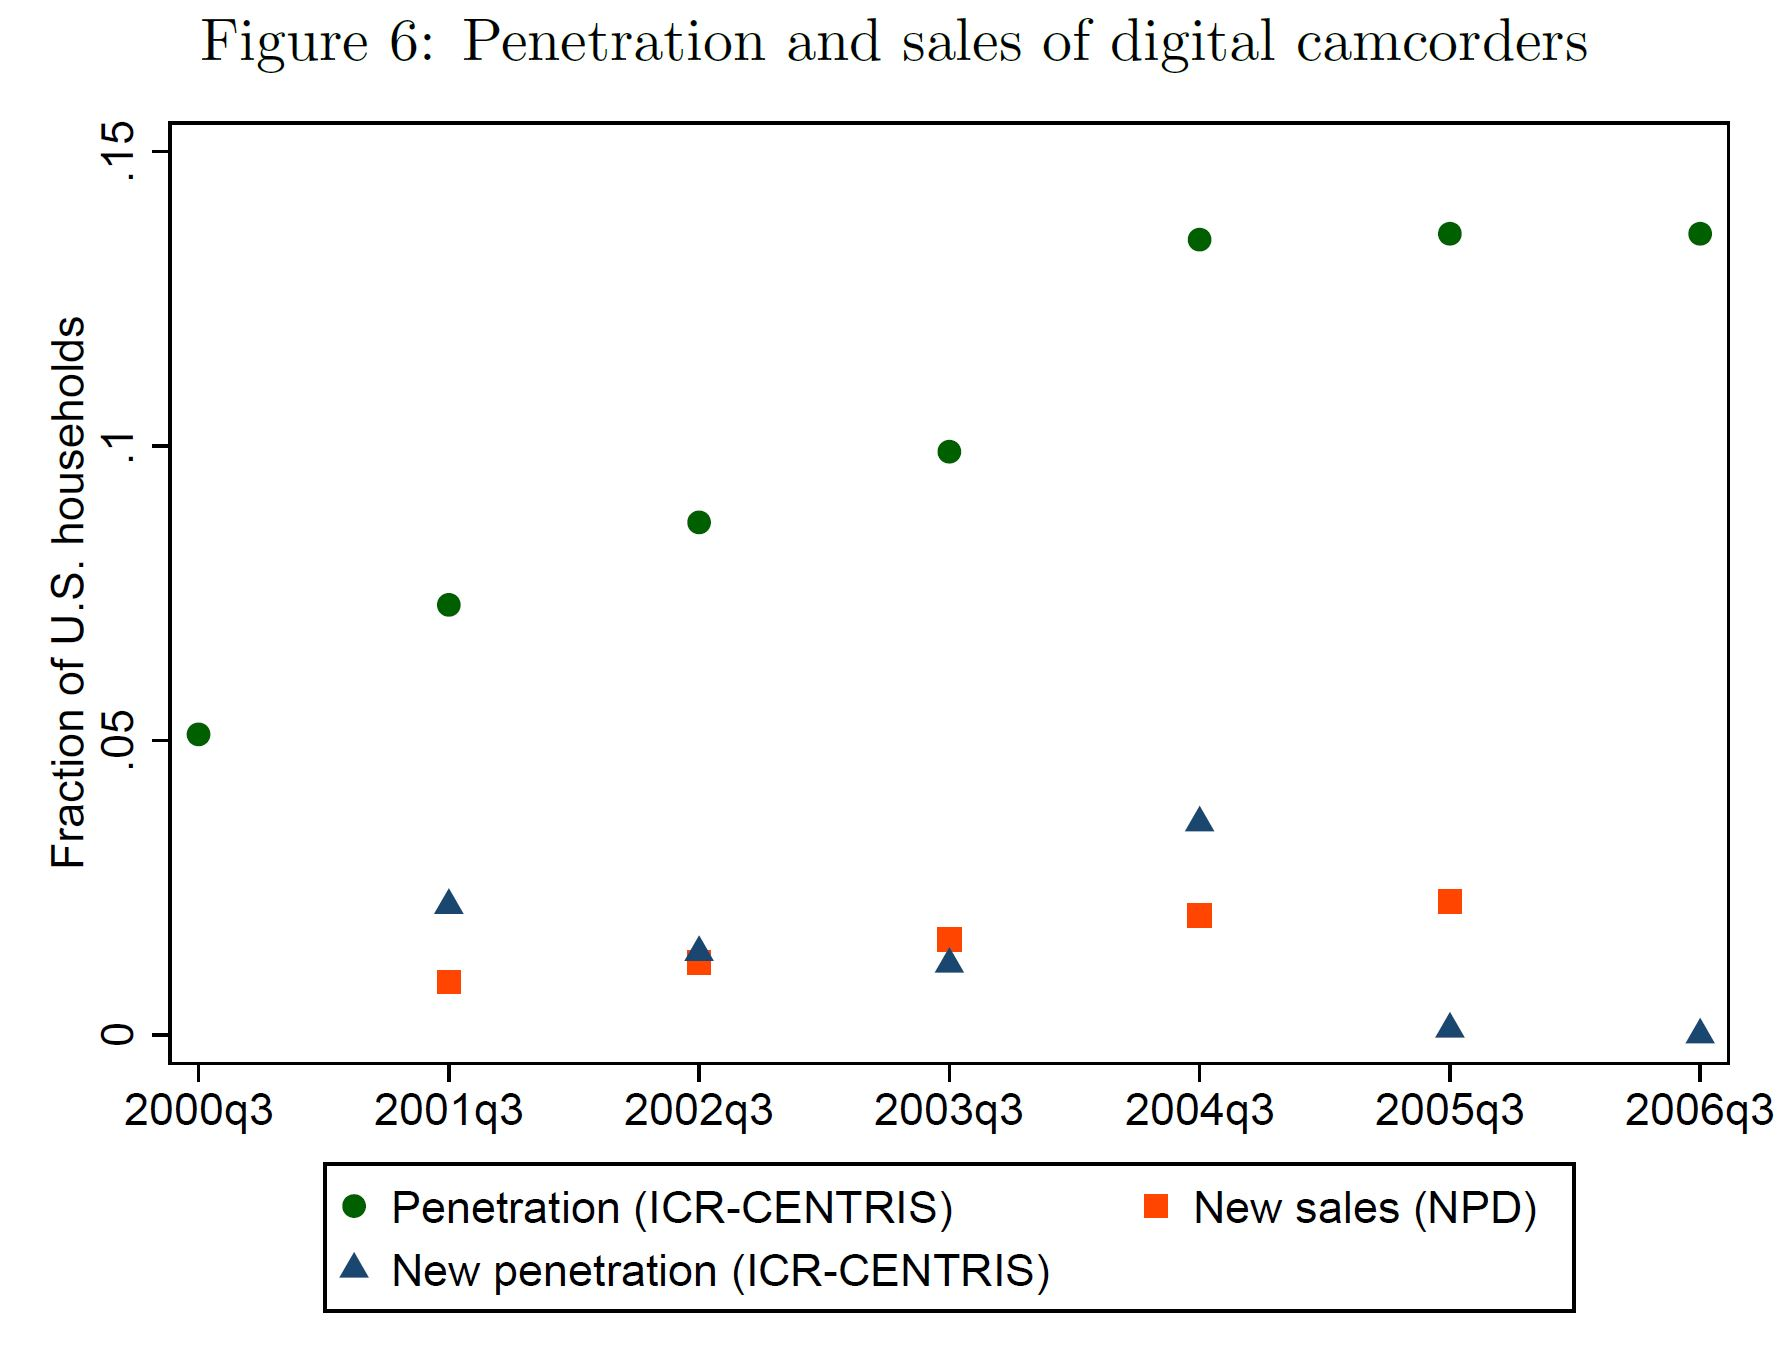
\includegraphics[width=\linewidth]{6.JPG}
  \end{figure}
\end{frame}

\begin{frame}
  \frametitle{Results}

  \begin{figure}
    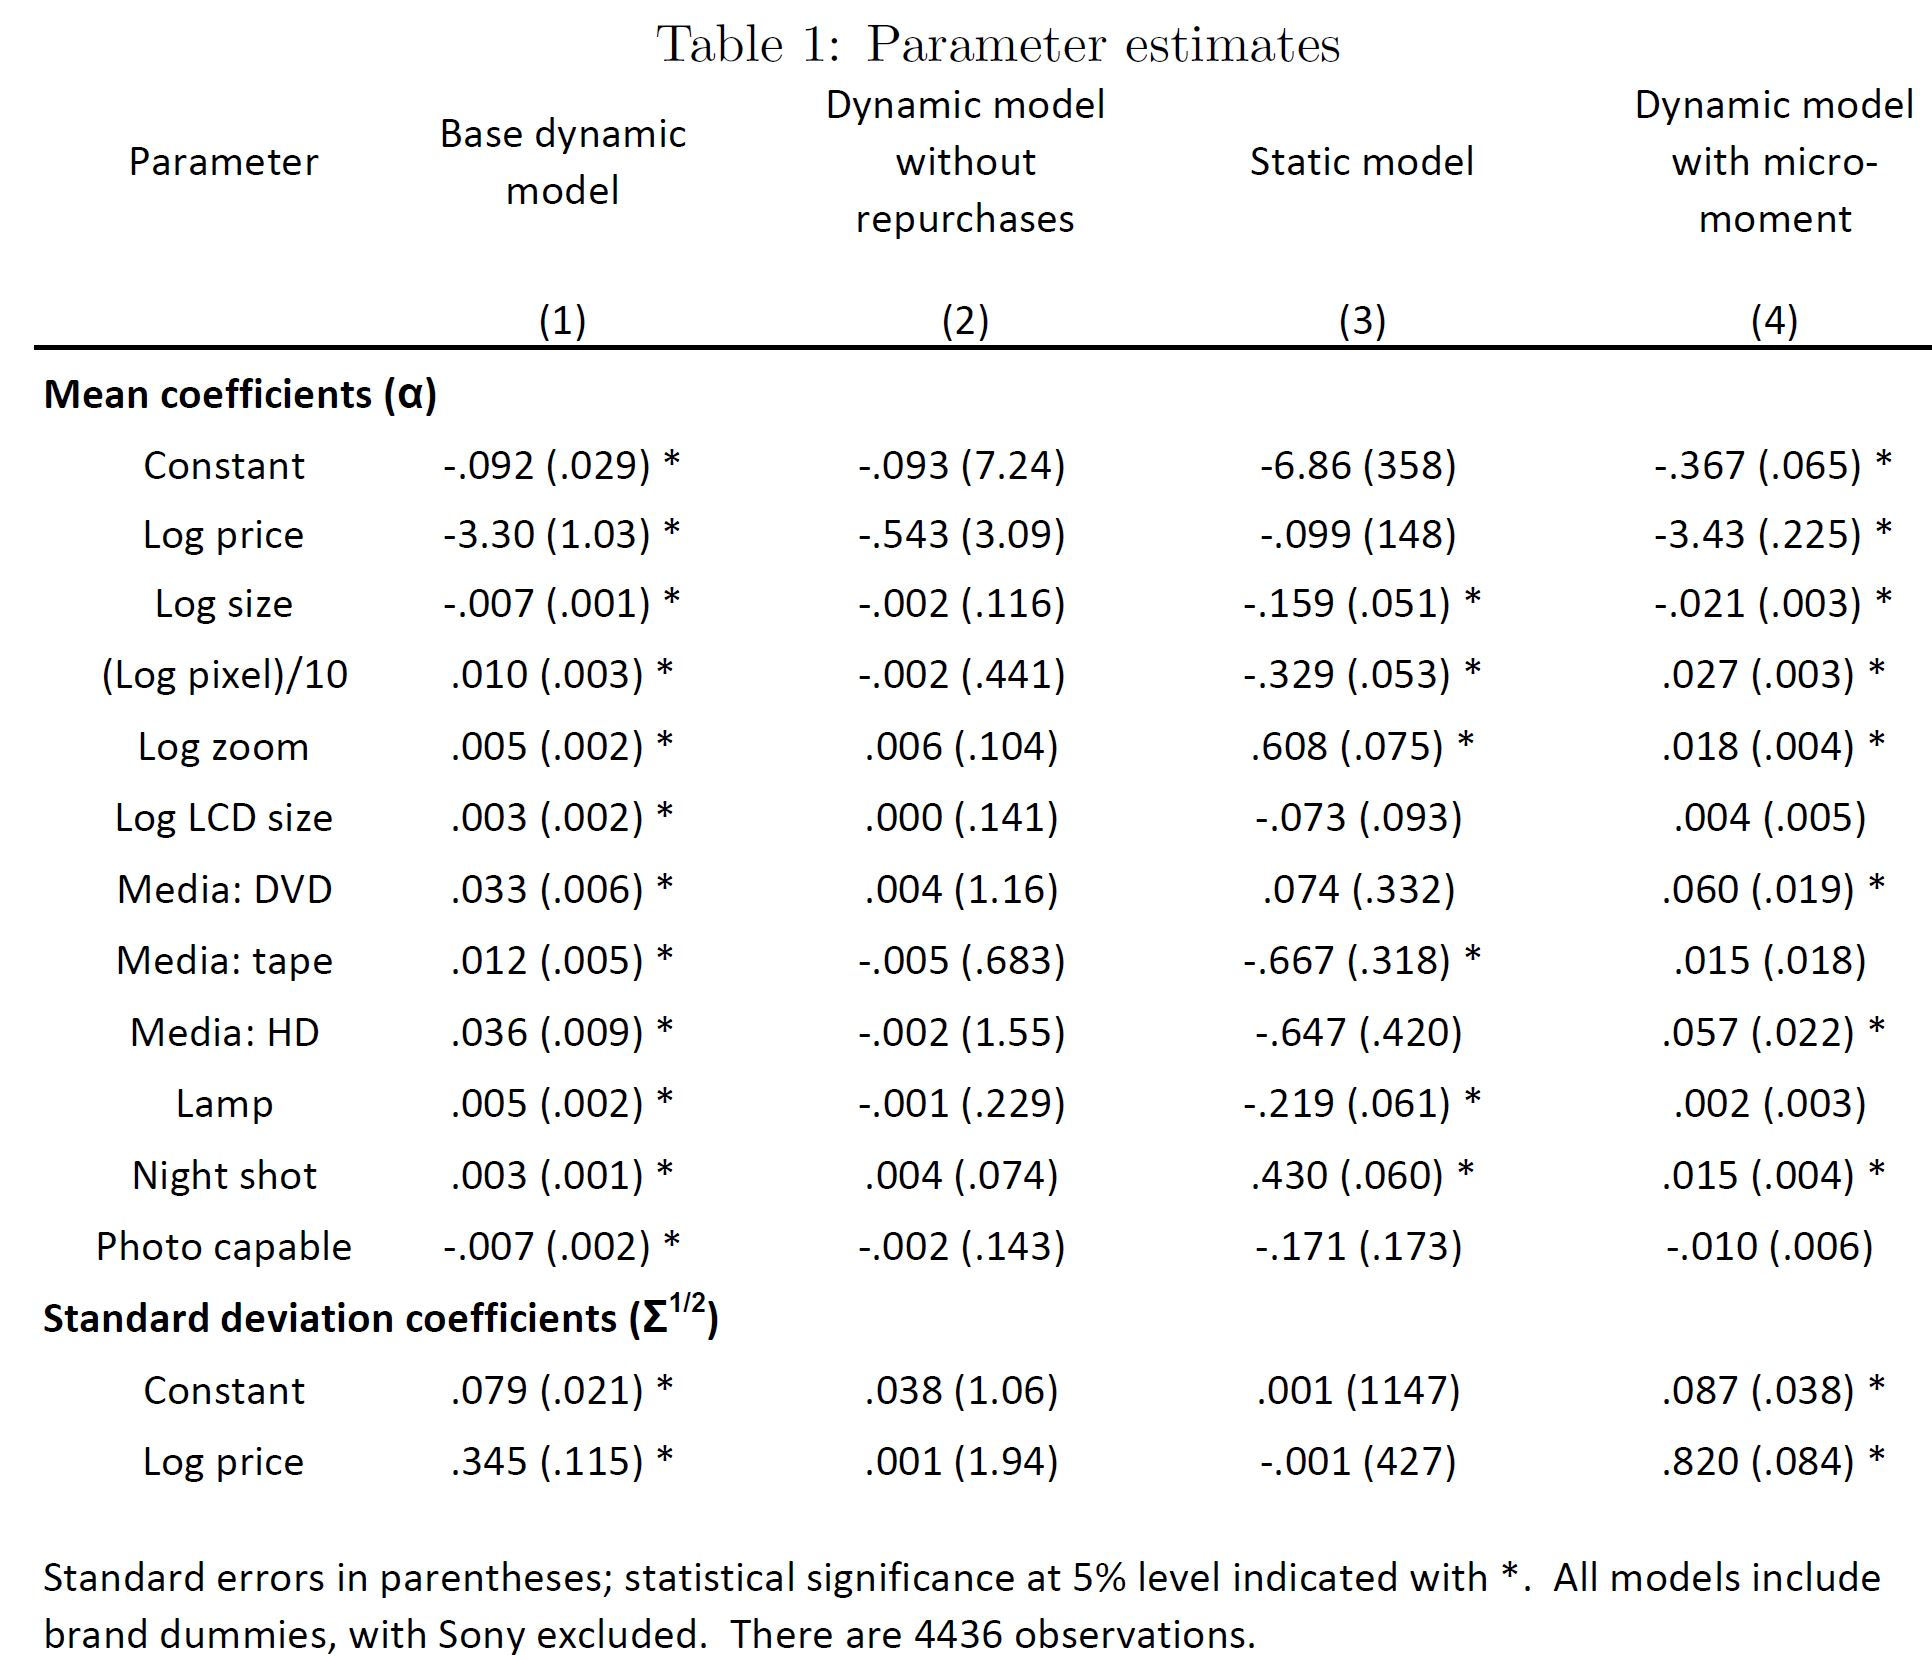
\includegraphics[width=\linewidth]{Table 1.JPG}
  \end{figure}
\end{frame}

\begin{frame}
  \frametitle{Results}

  \begin{itemize}
    \item Column 1 presents the results of or base model,
    \item Coefficients have the expected direction and are significant, that is,
      price decrease utility, quality measures increase utility.
    \item The low magnitude of quality coefficient are a consequence of the
      dynamic model and the coefficient are $(1 - \beta)$ times smaller than they
      would be in static model.
    \item Parameters on characteristics are smaller in absolute value than the
      constant term. This imply that difference between camcorders are small
      relative to the outside good.
  \end{itemize}
\end{frame}

\begin{frame}
  \frametitle{Results}

  \begin{itemize}
    \item Column 2 provides the same base model, but where individuals are
      restricted to purchase at most one digital camcorder ever,
    \item Column 2 coefficient are not reasonable.
    \item Column 3 shows the results in a static model, again coefficient
      are not reasonable, particularly price variance skyrocketed.
  \end{itemize}
\end{frame}

\begin{frame}
  \frametitle{Results}

  \begin{itemize}
    \item Even if Column 1 is significantly different from Column 2, repeating
      purchase represent only 0.25\% of total purchase.
    \item This is not consistent with evidence.
    \item Column 4 tries to address by matching repeating purchase with
      penetration data.
    \item Coefficients of Column 4 is consistent with the results in the Base model
  \end{itemize}
\end{frame}

\begin{frame}
  \frametitle{Results: Repeated purchase}

  \begin{figure}
    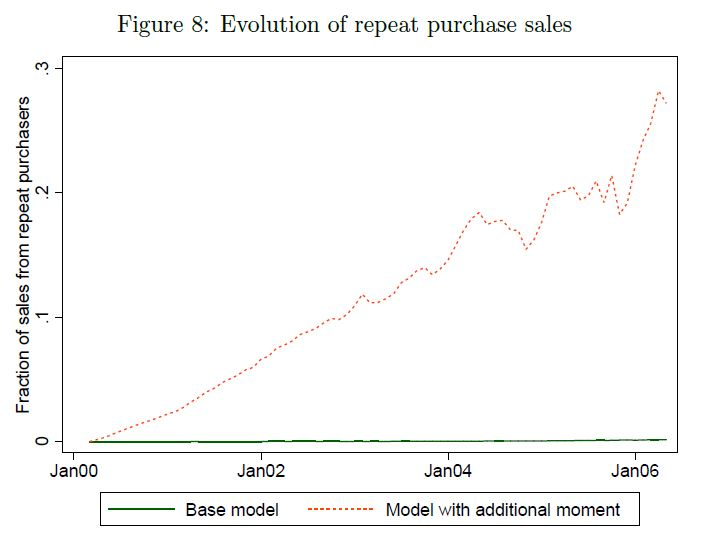
\includegraphics[width=\linewidth]{8.JPG}
  \end{figure}
\end{frame}

\begin{frame}
  \frametitle{Results: Logit error assumption}

  \begin{itemize}
    \item Logit error implies unrealistic welfare gain from new products,
    \item To test for it, we add $ln(J_t)$ as regressor. Finding a coefficient of $0$
      implies that logit model is well-specified, finding a coefficient of $-1$
      implies that is no demand expansion effect from variety,
    \item We find a value of $-0.013$ which is significantly different from $0$.
    \item But since "it is very close to zero" we conclude that the Logit Error
      assumption is reasonable.
  \end{itemize}
\end{frame}


%\begin{frame}
  %\frametitle{Results - Repeated Purchase}

  %\begin{itemize}
  %\item The base model projects a very low rate of repeated purchase, around $
    %0.25\%$
  %\item This in inconsistent with ICR dataset, 
%n\end{itemize}n
%\begin{frame}
  %\frametitle{Results - Repeated Purchase}


  %\begin{figure}
    %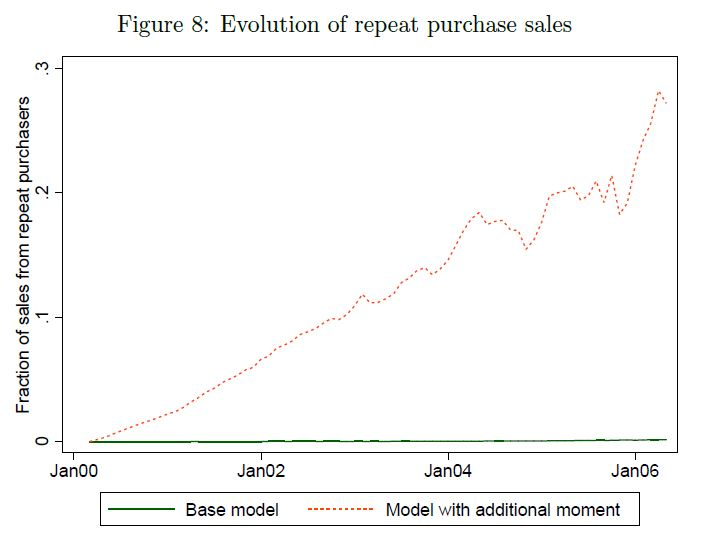
\includegraphics[width=\linewidth]{8.JPG}
  %\end{figure}
%\end{frame}

\begin{frame}
  \frametitle{Results: Comparitive analysis}

  \begin{itemize}
    \item If price and quality are assumed not to change market share have
      radically different behaviour
    \item If camcorder were not a durable good, to the surprise of consumers,
      market share would rise even faster.
  \end{itemize}

  \begin{figure}
    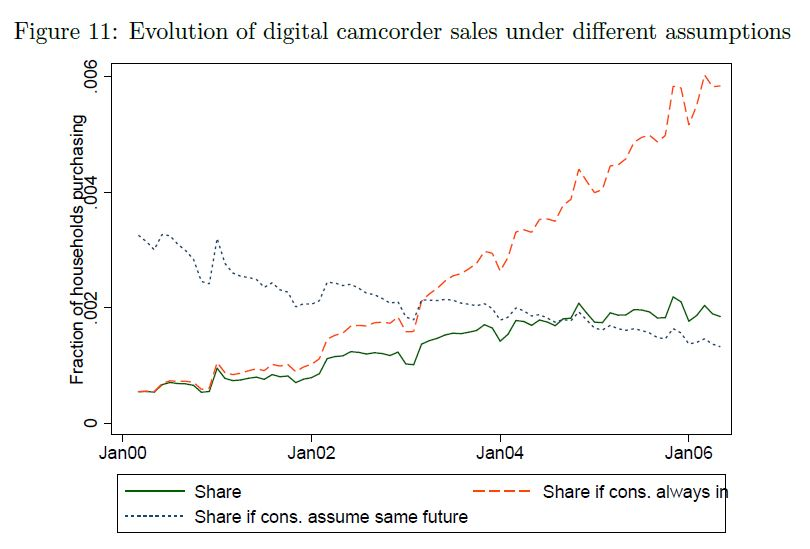
\includegraphics[width=\linewidth]{11.JPG}
  \end{figure}
\end{frame}

\begin{frame}
  \frametitle{Results: COLI}

  \begin{itemize}
    \item A new Cost of Living Index is derived from our dynamic model,
    \item This is done by measuring a compensating variation that makes the
      average expected value function to be constant over time,
    \item This new COLI substantially differ from standards CPIs measures,
    \item Which shows that the "news buyer problem", that is the fact the prices
      drop on durable goods disproportionally benefits consumers with lower
      evaluation, to be empirically important.
  \end{itemize}
  
\end{frame}

\begin{frame}
  \frametitle{Results: COLI}

  \begin{figure}
    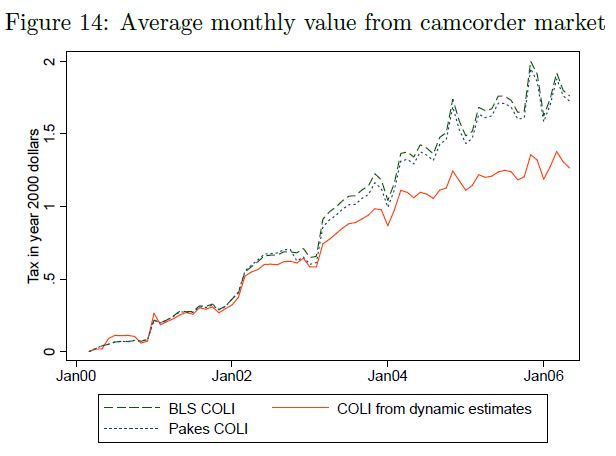
\includegraphics[width=\linewidth]{14.JPG}
  \end{figure}
\end{frame}

\begin{frame}
  \frametitle{Conclusion}
  
  \begin{itemize}
    \item The paper develop new methods to estimate dynamics of consumers preferences
      for new durable goods,
    \item The model can be used to measure welfare impact of new durable good,
    \item It's shown that initial market share for digital camcorders was not higher
      because of rational expectation of price and quality.
    \item Standard COLI's overstate the welfare gain of market evolution, because 
      ignore the fact that later adopters tend to value product less than earlier adopters.
  \end{itemize}

\end{frame}

\begin{frame}
  \frametitle{Extras}

  \begin{figure}
    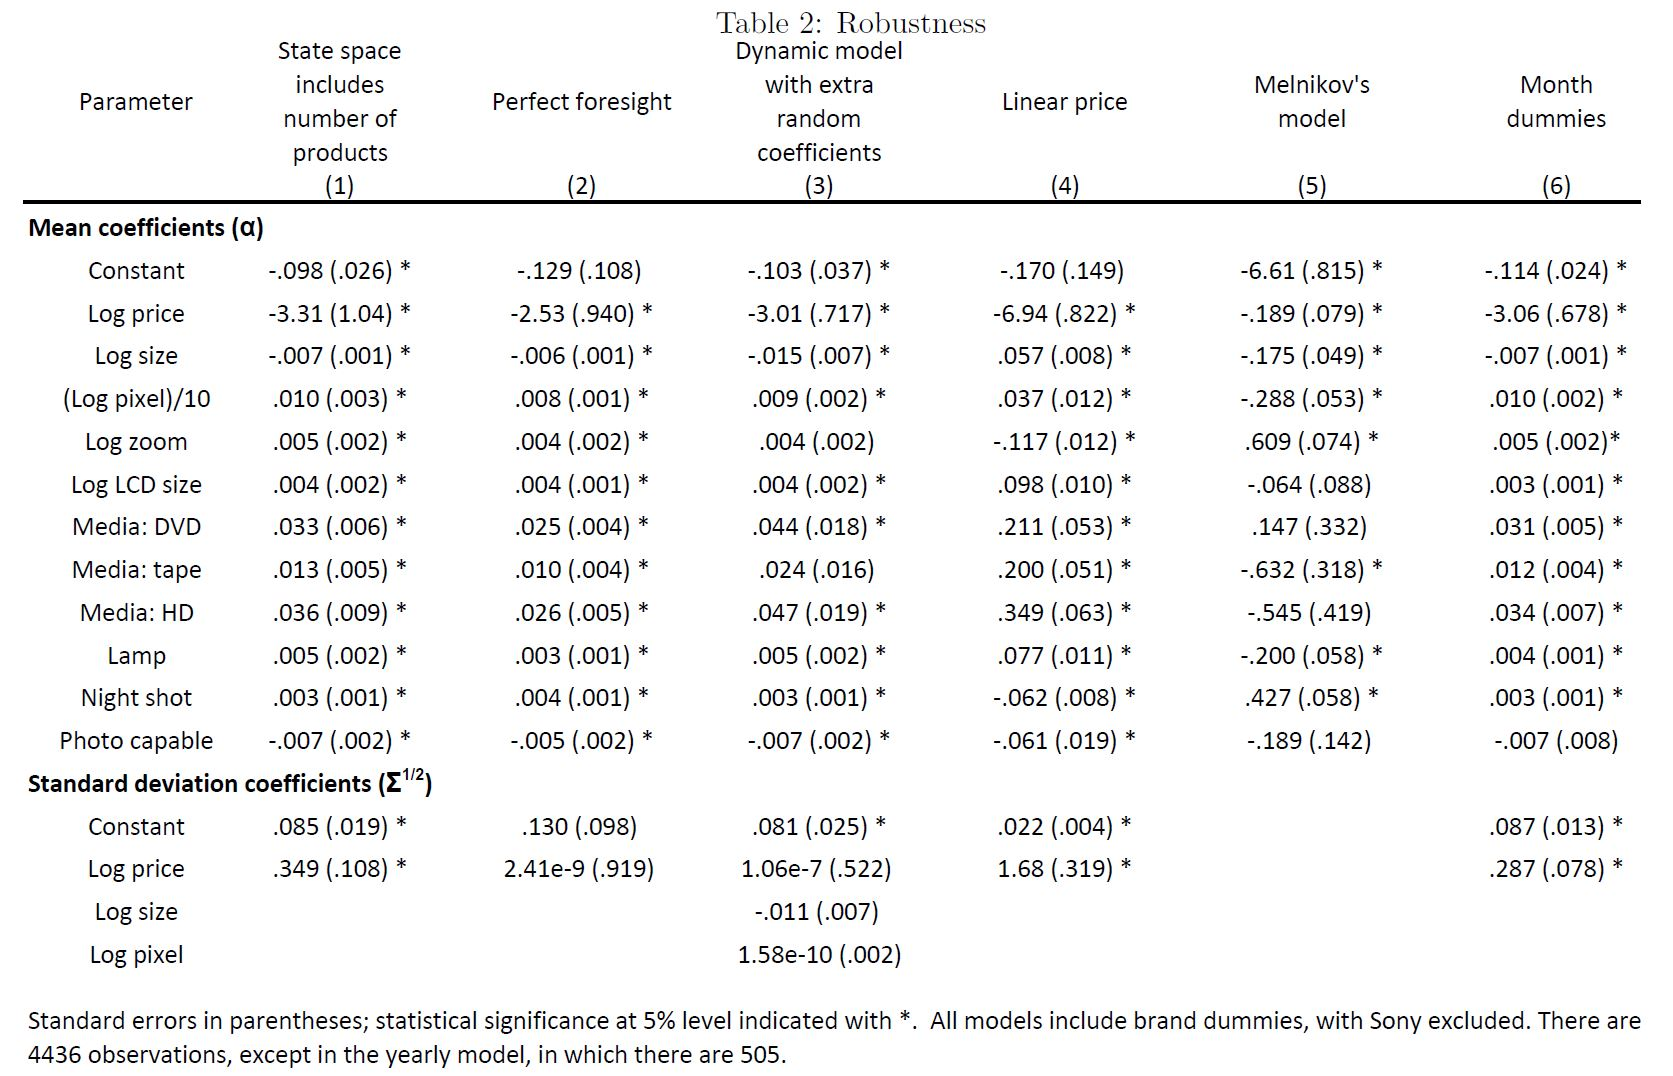
\includegraphics[width=\linewidth]{Table 2.JPG}
  \end{figure}
\end{frame}

\begin{frame}
  \frametitle{Extras}

  \begin{figure}
    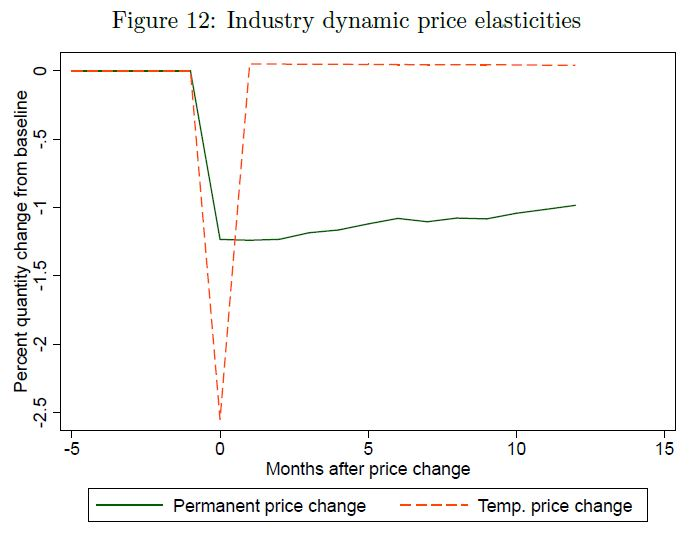
\includegraphics[width=\linewidth]{12.JPG}
  \end{figure}
\end{frame}

\begin{frame}
  \frametitle{Extras}

  \begin{figure}
    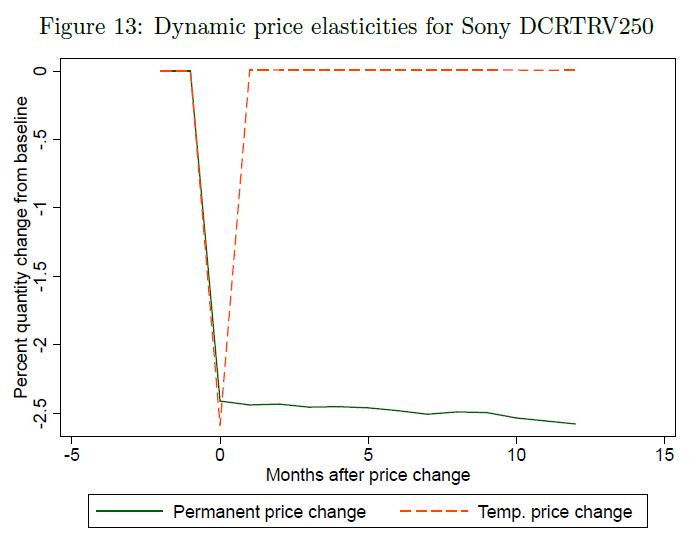
\includegraphics[width=\linewidth]{13.JPG}
  \end{figure}
\end{frame}

\begin{frame}
  \frametitle{Extras}

  \begin{figure}
    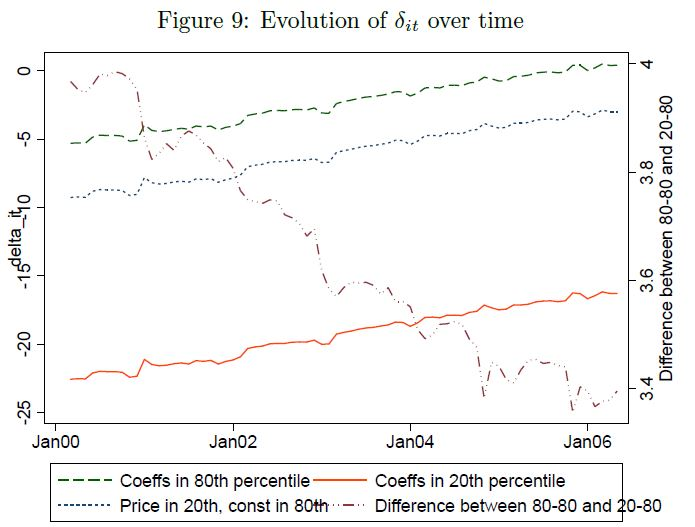
\includegraphics[width=\linewidth]{9.JPG}
  \end{figure}
\end{frame}
\end{document}
